\documentclass[9pt]{beamer}
\beamertemplatenavigationsymbolsempty
\usetikzlibrary{positioning}
\usepackage{subfig}
%\usetheme{Berlin}

\usepackage{etex, tikz, array, graphics, xspace, relsize, multirow}
\usepackage{ulem}

\input binhex

% For code inclusion
\usepackage{listings}
\lstset{ breaklines=true}
\lstset{escapeinside={<@}{@>}}
\usepackage{algorithm2e}
\usepackage{algorithmic}

% Commands
\newcommand\A{\mathcal{A}}
\newcommand\cc{\mathcal{C}}
\newcommand\codim{\mathrm{codim}}
\newcommand\CP{\mathbb{CP}}
\newcommand\C{\mathbb{C}}
\newcommand\D{\mathrm{D}}
\newcommand\hto{\hookrightarrow}
\newcommand\I{^{-1}}
\newcommand\oo{\mathcal{O}}
\renewcommand\phi{\varphi}
\newcommand\Pj{\mathbb{P}}
\newcommand\pow{\mathcal{P}}
\newcommand\RP{\mathbb{RP}}
\newcommand\rstr[2]{{\left.#1\right|_{#2}}}
\newcommand\R{\mathbb{R}}
\newcommand\V{\mathcal{V}}
\newcommand\F{\mathcal{F}}
\newcommand\G{\mathcal{G}}
\newcommand\Graph{\G(\F_{\mathcal{L}, b}, G)}
\newcommand\set[1]{\{#1\}}
\newcommand\toi{\xrightarrow{\sim}} % category
\newcommand\Z{\mathbb{Z}}


% For drawing
%% Tikz drawing
\usepackage{tikz}
\usetikzlibrary{arrows}
\usetikzlibrary{arrows.meta}
\usepackage{pgfplots}
\usepackage{tikz-3dplot}
\usepackage{tcolorbox}
\usetikzlibrary{matrix,fit,positioning,shapes.geometric,patterns,backgrounds}
\usetikzlibrary{decorations.pathreplacing}
\usetikzlibrary{decorations.markings}
\usetikzlibrary{arrows,calc}
\tikzstyle{bigbox} = [draw=blue!50, thick, rounded corners, rectangle]
\tikzset{
  >=stealth'
}
\tikzset{->-/.style={decoration={
      markings,
      mark=at position #1 with {\arrow{>}}},postaction={decorate}}}

%% Software names
\newcommand\topcom{\texttt{TOPCOM}\xspace}
\newcommand\mptopcom{\texttt{MPTOPCOM}\xspace}
\newcommand\mptopcomone{\texttt{MPTOPCOM-1}\xspace}
\newcommand\mts{\texttt{mts}\xspace}
\newcommand\mplrs{\texttt{mplrs}\xspace}
\newcommand\soplex{\texttt{soplex}\xspace}
\newcommand\openmpi{\texttt{OpenMPI}\xspace}
\newcommand\mpi{\texttt{MPI}\xspace}
\newcommand\gfan{\texttt{Gfan}\xspace}
\newcommand\cddlib{\texttt{cddlib}\xspace}
\newcommand\polydb{\texttt{PolyDB}\xspace}
\newcommand\OSCAR{\texttt{OSCAR}\xspace}
\newcommand\Julia{\texttt{Julia}\xspace}

\usepackage{xcolor}
\definecolor{green}{rgb}{0.1,0.59,0.1}
\definecolor{yellow}{rgb}{0.8,0.67,0}
\definecolor{red}{rgb}{0.89,0.1,0.1}
\definecolor{blue}{rgb}{0.1,0.1,0.89}

\usenavigationsymbolstemplate{}

\usepackage{booktabs}
% For software citations
\newcommand{\polymake}{\texttt{po\-ly\-ma\-ke}\xspace}
\newcommand{\polymakejl}{\texttt{Po\-ly\-ma\-ke.jl}\xspace}
\newcommand{\singular}{\texttt{Sin\-gu\-lar}\xspace}
\newcommand\CPP{C\nolinebreak\hspace{-.05em}\raisebox{.4ex}{\relsize{-3}{\textbf{+}}}\nolinebreak\hspace{-.10em}\raisebox{.4ex}{\relsize{-3}{\textbf{+}}}\xspace}

\usepackage{amsmath}
% Newcommands specifically for this article
\newcommand{\eval}{v}               % evaluation function giving switch table
\newcommand{\graph}{\Gamma}         % reverse search graph
\newcommand{\group}{G}              % group acting on point config
\newcommand{\groupElem}{g}          % element of group
\newcommand{\jbound}{\psi}          % bound on the number of elements of set J
\newcommand{\switchTableSize}{\mu}  % index of last non-trivial row in switch table

\newcommand{\pc}{\mathcal P\mathcal C}
\newcommand{\ZZ}{\mathbb Z}
\renewcommand{\AA}{\mathcal A}
\newcommand{\QQ}{\mathbb Q}
\newcommand{\OO}{\mathcal O}
\newcommand{\CC}{\mathbb C}
\newcommand{\PP}{\mathbb P}
\newcommand{\RR}{\mathbb R}
\newcommand{\scalp}[1]{\langle #1 \rangle}
\newcommand{\wt}{\omega}
\newcommand{\cT}{\mathcal T}
\renewcommand{\O}{\mathcal O}
\newcommand{\adm}{\mathcal A(\D, M)}
\newcommand{\blue}[1]{{\usebeamercolor[fg]{palette primary}#1}}

\DeclareMathOperator{\CaDiv}{CaDiv}
\DeclareMathOperator{\conv}{conv}
\DeclareMathOperator{\below}{defect}
\DeclareMathOperator{\vertex}{vertex}
\DeclareMathOperator{\Cox}{Cox}
\DeclareMathOperator{\cl}{cl}
\DeclareMathOperator{\cone}{cone}
\DeclareMathOperator{\Ext}{Ext}
\DeclareMathOperator{\Tor}{Tor}
\DeclareMathOperator{\lcm}{lcm}
\DeclareMathOperator{\Quot}{Quot}
\DeclareMathOperator{\Spec}{Spec}
\DeclareMathOperator{\Sets}{Sets}
\DeclareMathOperator{\relint}{relint}
\DeclareMathOperator{\rk}{rk}
\DeclareMathOperator{\smallestFace}{smallestFace}
\DeclareMathOperator{\Pic}{Pic}
\DeclareMathOperator{\Hom}{Hom}
\DeclareMathOperator{\vol}{vol}
\DeclareMathOperator{\TV}{TV}
\DeclareMathOperator{\tail}{tail}
\DeclareMathOperator{\rep}{rep}
\DeclareMathOperator{\vspan}{span}
\DeclareMathOperator{\canonical}{can}
\DeclareMathOperator{\gkz}{gkz}

\newcommand{\pmsmall}{
\includegraphics[scale=0.03]{pmlogo.png}}
\newcommand{\pmlogo}{
\includegraphics[scale=0.09]{pmlogo.png}}
\newcommand{\pmbluesmall}{\includegraphics[scale=0.03]{pmbluelogo.png}}
\newcommand{\Disjoint}{\mathop{\coprod}}
\newcommand{\Discriminant}{\mathcal{D}}

\theoremstyle{definition}
\newtheorem{remark}{Remark}

\newtheorem{lem}{Lemma}
\newtheorem{defn}{Definition}

\author[Antony Della Vecchia]{Antony Della Vecchia \\ \vspace{4mm} \small{Joint work with F. Lenzen and M. Joswig } }
\title{Partial Algebraic Shifting}

\institute[]{
  TU Berlin
}
\date{

  2025-06-03
}
\logo{
  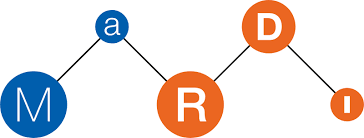
\includegraphics[width=2cm]{images/mardi-logo.png}
}


\newcommand{\surj}{\twoheadrightarrow}
\newcommand{\oursetting}[1]{\textcolor{blue}{#1}}
\usepackage{listings}
\begin{document}
\maketitle
%%%%%%%%%%%%%%%%%%%%%%%%%%%%%%%%%%%%%%%%%%%%%%%%%%%%%%%%%%%%%%%%%%%%%%%%%%%%%%% 
%%%%%%%%%%%%%%%%%%%%%%%%%%%%%%%%%%%%%%%%%%%%%%%%%%%%%%%%%%%%%%%%%%%%%%%%%%%%%%% 
%%%%%%%%%%%%%%%%%%%%%%%%%%%%%%%%%%%%%%%%%%%%%%%%%%%%%%%%%%%%%%%%%%%%%%%%%%%%%%% 


\begin{frame}[fragile]{Algebraic Shifting motivation}
  %  \begin{itemize}
  %  \item f vector and betti number
  %  \item near cone
  %  \item classifying betti and f vector sequences
  %  \item rigidity?
  %  \end{itemize}
  \begin{figure}[h!]
    \centering
    \subfloat{\tikz[remember picture]{\node(1AL){
          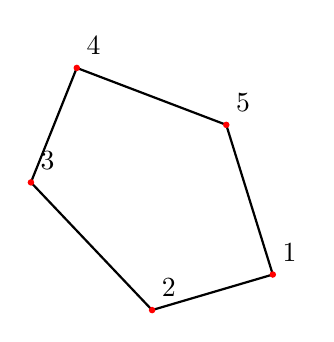
\begin{tikzpicture}

            % DEF COORDINATES
            \coordinate (v0_unnamed__1) at (1.33661, -1.24914, -0.520718);
            \coordinate (v1_unnamed__1) at (0.605842, -0.898371, 1.5633);
            \coordinate (v2_unnamed__1) at (-0.962171, 0.693911, 1.48688);
            \coordinate (v3_unnamed__1) at (-1.2005, 1.32724, -0.64435);
            \coordinate (v4_unnamed__1) at (0.220225, 0.126361, -1.88511);


            % VERTEXCOLOR
            \definecolor{vertexcolor_unnamed__1}{rgb}{ 1 0 0 }

            % DEF VERTEXSTYLES
            \tikzstyle{vertexstyle_unnamed__1_0} = [circle, scale=0.25, fill=vertexcolor_unnamed__1,label={[text=black, above right, align=left]:1},]
            \tikzstyle{vertexstyle_unnamed__1_1} = [circle, scale=0.25, fill=vertexcolor_unnamed__1,label={[text=black, above right, align=left]:2},]
            \tikzstyle{vertexstyle_unnamed__1_2} = [circle, scale=0.25, fill=vertexcolor_unnamed__1,label={[text=black, above right, align=left]:3},]
            \tikzstyle{vertexstyle_unnamed__1_3} = [circle, scale=0.25, fill=vertexcolor_unnamed__1,label={[text=black, above right, align=left]:4},]
            \tikzstyle{vertexstyle_unnamed__1_4} = [circle, scale=0.25, fill=vertexcolor_unnamed__1,label={[text=black, above right, align=left]:5},]

            % EDGECOLOR
            \definecolor{edgecolor_unnamed__1}{rgb}{ 0 0 0 }
            \tikzstyle{edgestyle_unnamed__1} = [thick,color=edgecolor_unnamed__1]

            % EDGES

            \foreach \i/\k in {1/0,2/1,3/2,4/0,4/3} {
              \draw[edgestyle_unnamed__1] (v\i_unnamed__1) -- (v\k_unnamed__1);
            }


            % POINTS
            \foreach \i in {1,2,0,3,4} {
              \node at (v\i_unnamed__1) [vertexstyle_unnamed__1_\i] {};
            }


          \end{tikzpicture}
        }%
        \hspace*{3cm}%
        \subfloat{\tikz[remember picture]{\node(1AR){
              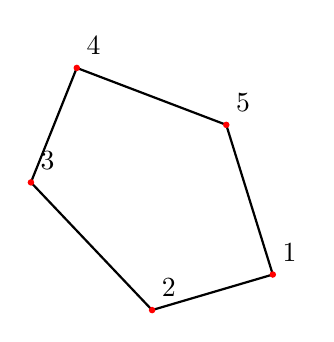
\begin{tikzpicture}

                % DEF COORDINATES
                \coordinate (v0_unnamed__1) at (1.33661, -1.24914, -0.520718);
                \coordinate (v1_unnamed__1) at (0.605842, -0.898371, 1.5633);
                \coordinate (v2_unnamed__1) at (-0.962171, 0.693911, 1.48688);
                \coordinate (v3_unnamed__1) at (-1.2005, 1.32724, -0.64435);
                \coordinate (v4_unnamed__1) at (0.220225, 0.126361, -1.88511);


                % VERTEXCOLOR
                \definecolor{vertexcolor_unnamed__1}{rgb}{ 1 0 0 }

                % DEF VERTEXSTYLES
                \tikzstyle{vertexstyle_unnamed__1_0} = [circle, scale=0.25, fill=vertexcolor_unnamed__1,label={[text=black, above right, align=left]:1},]
                \tikzstyle{vertexstyle_unnamed__1_1} = [circle, scale=0.25, fill=vertexcolor_unnamed__1,label={[text=black, above right, align=left]:2},]
                \tikzstyle{vertexstyle_unnamed__1_2} = [circle, scale=0.25, fill=vertexcolor_unnamed__1,label={[text=black, above right, align=left]:3},]
                \tikzstyle{vertexstyle_unnamed__1_3} = [circle, scale=0.25, fill=vertexcolor_unnamed__1,label={[text=black, above right, align=left]:4},]
                \tikzstyle{vertexstyle_unnamed__1_4} = [circle, scale=0.25, fill=vertexcolor_unnamed__1,label={[text=black, above right, align=left]:5},]

                % EDGECOLOR
                \definecolor{edgecolor_unnamed__1}{rgb}{ 0 0 0 }
                \tikzstyle{edgestyle_unnamed__1} = [thick,color=edgecolor_unnamed__1]

                % EDGES

                \foreach \i/\k in {1/0,2/1,3/2,4/0,4/3} {
                  \draw[edgestyle_unnamed__1] (v\i_unnamed__1) -- (v\k_unnamed__1);
                }


                % POINTS
                \foreach \i in {1,2,0,3,4} {
                  \node at (v\i_unnamed__1) [vertexstyle_unnamed__1_\i] {};
                }


              \end{tikzpicture}
  }}
\end{figure}
\tikz[overlay,remember picture]{\draw[-latex,thick] (1AL) -- (1AL-|1AR.west)
node[midway,below,text width=2.5cm]{Physical Line Graph Transformation};} 

  

\end{frame}


%%%%%%%%%%%%%%%%%%%%%%%%%%%%%%%%%%%%%%%%%%%%%%%%%%%%%%%%%%%%%%%%%%%%%%%%%%%%%%% 
%%%%%%%%%%%%%%%%%%%%%%%%%%%%%%%%%%%%%%%%%%%%%%%%%%%%%%%%%%%%%%%%%%%%%%%%%%%%%%% 
%%%%%%%%%%%%%%%%%%%%%%%%%%%%%%%%%%%%%%%%%%%%%%%%%%%%%%%%%%%%%%%%%%%%%%%%%%%%%%% 

\begin{frame}[fragile]{Algebraic Shifting constructions}
  \begin{itemize}
  \item shifted families
  \item explain the change of basis algorithm
  \item mention monte carlo and issues with finite characteristic
  \end{itemize}
\end{frame}

%%%%%%%%%%%%%%%%%%%%%%%%%%%%%%%%%%%%%%%%%%%%%%%%%%%%%%%%%%%%%%%%%%%%%%%%%%%%%%% 
%%%%%%%%%%%%%%%%%%%%%%%%%%%%%%%%%%%%%%%%%%%%%%%%%%%%%%%%%%%%%%%%%%%%%%%%%%%%%%% 
%%%%%%%%%%%%%%%%%%%%%%%%%%%%%%%%%%%%%%%%%%%%%%%%%%%%%%%%%%%%%%%%%%%%%%%%%%%%%%% 

\begin{frame}[fragile]{different perspectives }
  \begin{itemize}
  \item GIN
  \item plucker
  \item pick one and spell it out
  \end{itemize}
\end{frame}

%%%%%%%%%%%%%%%%%%%%%%%%%%%%%%%%%%%%%%%%%%%%%%%%%%%%%%%%%%%%%%%%%%%%%%%%%%%%%%% 
%%%%%%%%%%%%%%%%%%%%%%%%%%%%%%%%%%%%%%%%%%%%%%%%%%%%%%%%%%%%%%%%%%%%%%%%%%%%%%% 
%%%%%%%%%%%%%%%%%%%%%%%%%%%%%%%%%%%%%%%%%%%%%%%%%%%%%%%%%%%%%%%%%%%%%%%%%%%%%%% 

\begin{frame}[fragile]{Partial Algebraic Shifting }
  \begin{itemize}
  \item loose definition as a way to replace the generic matrix with a matrix that is parametrized by weyl group elements
  \item state result about standard n cycle
  \end{itemize}
\end{frame}

%%%%%%%%%%%%%%%%%%%%%%%%%%%%%%%%%%%%%%%%%%%%%%%%%%%%%%%%%%%%%%%%%%%%%%%%%%%%%%% 
%%%%%%%%%%%%%%%%%%%%%%%%%%%%%%%%%%%%%%%%%%%%%%%%%%%%%%%%%%%%%%%%%%%%%%%%%%%%%%% 
%%%%%%%%%%%%%%%%%%%%%%%%%%%%%%%%%%%%%%%%%%%%%%%%%%%%%%%%%%%%%%%%%%%%%%%%%%%%%%% 

\begin{frame}[fragile]{Real Projective Plane Example}
  \begin{itemize}
  \item show example of how we can compute full shift og projective plane with standard n cycle
  \item computations inspired us to find result
  \item example shows that our result is tight
  \end{itemize}
\end{frame}


%%%%%%%%%%%%%%%%%%%%%%%%%%%%%%%%%%%%%%%%%%%%%%%%%%%%%%%%%%%%%%%%%%%%%%%%%%%%%%% 
%%%%%%%%%%%%%%%%%%%%%%%%%%%%%%%%%%%%%%%%%%%%%%%%%%%%%%%%%%%%%%%%%%%%%%%%%%%%%%% 
%%%%%%%%%%%%%%%%%%%%%%%%%%%%%%%%%%%%%%%%%%%%%%%%%%%%%%%%%%%%%%%%%%%%%%%%%%%%%%% 

\begin{frame}[fragile]{LU decomposition and Bruhat decomposition }
  \begin{itemize}
  \item $\Delta_{gb}(K) = \Delta_g(K)$ for any upper triangular $b$
  \item $w_0g = lu = w_0u'w_0u$ (bring the two decompositions together)
  \item $u'w_0$ uses only $\frac{1}{2}n(n-1)$ transcendentals, which is a huge win computationally
  \item can we do better?
  \end{itemize}
\end{frame}

%%%%%%%%%%%%%%%%%%%%%%%%%%%%%%%%%%%%%%%%%%%%%%%%%%%%%%%%%%%%%%%%%%%%%%%%%%%%%%% 
%%%%%%%%%%%%%%%%%%%%%%%%%%%%%%%%%%%%%%%%%%%%%%%%%%%%%%%%%%%%%%%%%%%%%%%%%%%%%%% 
%%%%%%%%%%%%%%%%%%%%%%%%%%%%%%%%%%%%%%%%%%%%%%%%%%%%%%%%%%%%%%%%%%%%%%%%%%%%%%% 

\begin{frame}[fragile]{Inversions and Rothe matrix}
  \begin{itemize}
  \item Want a normal for Bw where B has minimal transcendentals.
  \item define inversions and show an example of how we we can remove transcendentals on the left.
  \item example of how to create a rothe matrix in Oscar
  \end{itemize}
\end{frame}


%%%%%%%%%%%%%%%%%%%%%%%%%%%%%%%%%%%%%%%%%%%%%%%%%%%%%%%%%%%%%%%%%%%%%%%%%%%%%%% 
%%%%%%%%%%%%%%%%%%%%%%%%%%%%%%%%%%%%%%%%%%%%%%%%%%%%%%%%%%%%%%%%%%%%%%%%%%%%%%% 
%%%%%%%%%%%%%%%%%%%%%%%%%%%%%%%%%%%%%%%%%%%%%%%%%%%%%%%%%%%%%%%%%%%%%%%%%%%%%%% 

\begin{frame}[fragile]{ Near cones}
  \begin{itemize}
  \item definition of near cone
  \item formula for computing their betti numbers
  \item State lemma about shifting to near cones
  \end{itemize}
\end{frame}

%%%%%%%%%%%%%%%%%%%%%%%%%%%%%%%%%%%%%%%%%%%%%%%%%%%%%%%%%%%%%%%%%%%%%%%%%%%%%%% 
%%%%%%%%%%%%%%%%%%%%%%%%%%%%%%%%%%%%%%%%%%%%%%%%%%%%%%%%%%%%%%%%%%%%%%%%%%%%%%% 
%%%%%%%%%%%%%%%%%%%%%%%%%%%%%%%%%%%%%%%%%%%%%%%%%%%%%%%%%%%%%%%%%%%%%%%%%%%%%%% 

\begin{frame}[fragile]{Shifting to Near cones proof}
  \begin{itemize}
  \item sketch proof extending permutation lemma
  \end{itemize}
\end{frame}

%%%%%%%%%%%%%%%%%%%%%%%%%%%%%%%%%%%%%%%%%%%%%%%%%%%%%%%%%%%%%%%%%%%%%%%%%%%%%%% 
%%%%%%%%%%%%%%%%%%%%%%%%%%%%%%%%%%%%%%%%%%%%%%%%%%%%%%%%%%%%%%%%%%%%%%%%%%%%%%% 
%%%%%%%%%%%%%%%%%%%%%%%%%%%%%%%%%%%%%%%%%%%%%%%%%%%%%%%%%%%%%%%%%%%%%%%%%%%%%%% 

\begin{frame}[fragile]{Weak Bruhat order}
  \begin{itemize}
  \item definition and equivalent formulation
  \item an example with rothe matrix that shows shifting to near cones
  \end{itemize}
\end{frame}

%%%%%%%%%%%%%%%%%%%%%%%%%%%%%%%%%%%%%%%%%%%%%%%%%%%%%%%%%%%%%%%%%%%%%%%%%%%%%%% 
%%%%%%%%%%%%%%%%%%%%%%%%%%%%%%%%%%%%%%%%%%%%%%%%%%%%%%%%%%%%%%%%%%%%%%%%%%%%%%% 
%%%%%%%%%%%%%%%%%%%%%%%%%%%%%%%%%%%%%%%%%%%%%%%%%%%%%%%%%%%%%%%%%%%%%%%%%%%%%%% 

\begin{frame}[fragile]{Proof of results}
  \begin{itemize}
  \item state proposition 25
  \item sketch proof
  \end{itemize}
\end{frame}


%%%%%%%%%%%%%%%%%%%%%%%%%%%%%%%%%%%%%%%%%%%%%%%%%%%%%%%%%%%%%%%%%%%%%%%%%%%%%%% 
%%%%%%%%%%%%%%%%%%%%%%%%%%%%%%%%%%%%%%%%%%%%%%%%%%%%%%%%%%%%%%%%%%%%%%%%%%%%%%% 
%%%%%%%%%%%%%%%%%%%%%%%%%%%%%%%%%%%%%%%%%%%%%%%%%%%%%%%%%%%%%%%%%%%%%%%%%%%%%%% 

\begin{frame}[fragile]{Mardi slide?}
  \begin{itemize}
  \item talk about how file format was useful
  \end{itemize}
\end{frame}

%%%%%%%%%%%%%%%%%%%%%%%%%%%%%%%%%%%%%%%%%%%%%%%%%%%%%%%%%%%%%%%%%%%%%%%%%%%%%%% 
%%%%%%%%%%%%%%%%%%%%%%%%%%%%%%%%%%%%%%%%%%%%%%%%%%%%%%%%%%%%%%%%%%%%%%%%%%%%%%% 
%%%%%%%%%%%%%%%%%%%%%%%%%%%%%%%%%%%%%%%%%%%%%%%%%%%%%%%%%%%%%%%%%%%%%%%%%%%%%%% 

\begin{frame}[fragile]{}
  \begin{center}
    QR codes to both papers

    Thank You!
  \end{center}
\end{frame}

%%%%%%%%%%%%%%%%%%%%%%%%%%%%%%%%%%%%%%%%%%%%%%%%%%%%%%%%%%%%%%%%%%%%%%%%%%%%%%%
%%%%%%%%%%%%%%%%%%%%%%%%%%%%%%%%%%%%%%%%%%%%%%%%%%%%%%%%%%%%%%%%%%%%%%%%%%%%%%%
%%%%%%%%%%%%%%%%%%%%%%%%%%%%%%%%%%%%%%%%%%%%%%%%%%%%%%%%%%%%%%%%%%%%%%%%%%%%%%%

\end{document}
